\subsubsection*{\textit{Explanation of simulation-based models}}

A simulator-based model is a parameterised stochastic data generating
mechanism \autocite{Gutmann2016}. The key characteristic of these
models is that although we can sample (simulate) data points, we
cannot evaluate the likelihood for a specific set of observations
$\data$. Formally, a simulator-based model is described as a
parameterised family of probability density functions
$\{ p_{\yb|\thetab}(\yb) \}_{\thetab}$, whose closed-form is either
unknown or intractable to evaluate. Whereas evaluating
$p_{\yb|\thetab}(\yb)$ is intractable, sampling is
feasible. Practically, a simulator can be understood as a black-box
machine $M_r$\footnote{The subscript $r$ in $M_r$ indicates the
  \textit{random} simulator. In the next chapters we will introduce
  $M_d$ witch stands for the \textit{deterministic} simulator.} that
given a set of parameters $\thetab$, produces samples $\yb$ in a
stochastic manner i.e.\ $M_r(\thetab) \rightarrow \yb$.

Simulator-based models are particularly captivating due to the
modelling freedom they provide; any physical process that can be
conceptualised as a computer program of finite (deterministic or
stochastic) steps can be modelled as a simulator-based model without
any compromise. The modelling fredom includes any amount of hidden
(unobserved) internal variables or logic-based decisions. As always,
this degree of freedom comes at a cost; performing the inference is
particularly demanding from both computational and mathematical
perspective. Unfortunately, the algorithms deployed so far permit the
inference only at low-dimensionality parametric spaces, i.e.\
$\thetab \in \mathbb{R}^D$ where $D$ is small.

\subsubsection*{\textit{Example}}

For underlying the importance of simulator-based models, let us use
the tuberculosis disease spread example as described in
\autocite{Tanaka2006}. An overview of the disease spread model is
presented at figure~\ref{fig:tuberculosis_model}. At each stage one of
the following \textit{unobserved} events may happen; (a) the
transmission of a specific haplotype to a new host, (b) the mutation
of an existent haplotype or (c) the exclusion of an infectious host
(recovers/dies) from the population. The random process, which stops
when $m$ infectious hosts are reached\footnote{We suppose that the
  unaffected population is infinite, so a new host can always be added
  until we reach $m$ simultaneous hosts.}, can be parameterised by the
transmission rate $\alpha$, the mutation rate $\tau$ and the exclusion
rate $\delta$, creating a $3D$-parametric space
$\thetab = (\alpha, \tau, \delta)$. The outcome of the process is a
variable-size tuple $\yb_{\thetab}$, containing the population
contaminated by each different haplotype, as described in
figure~\ref{fig:tuberculosis_model}. Lets say that the disease has
been spread in a real population and when $m$ hosts where contaminated
simultaneously, the vector with the infectious populations has been
measured to be $\data$. We would like to discover the parameters
$\thetab = (\alpha, \tau, \delta)$ that describe the spreading process
and lead to the specific outcome $\data$. Computing
$p(\yb=\data|\thetab)$ requires tracking all tree-paths that could
generate the specific tuple; such exhaustive enumeration becomes
intractable when $m$ grows larger, as in real-case scenarios. In
figure~\ref{fig:tuberculosis_model} we can observe that a transmission
followed by a recovery/death creates a loop, reinstating the process
to the previous step, which also ... the exhaustive
enumeration. Hence, modelling the process as a simulator-based
model\footnote{which is simple and efficient} and performing
likelihood-free inference is the suggested solution.

\begin{figure}[!ht]
    \begin{center}
      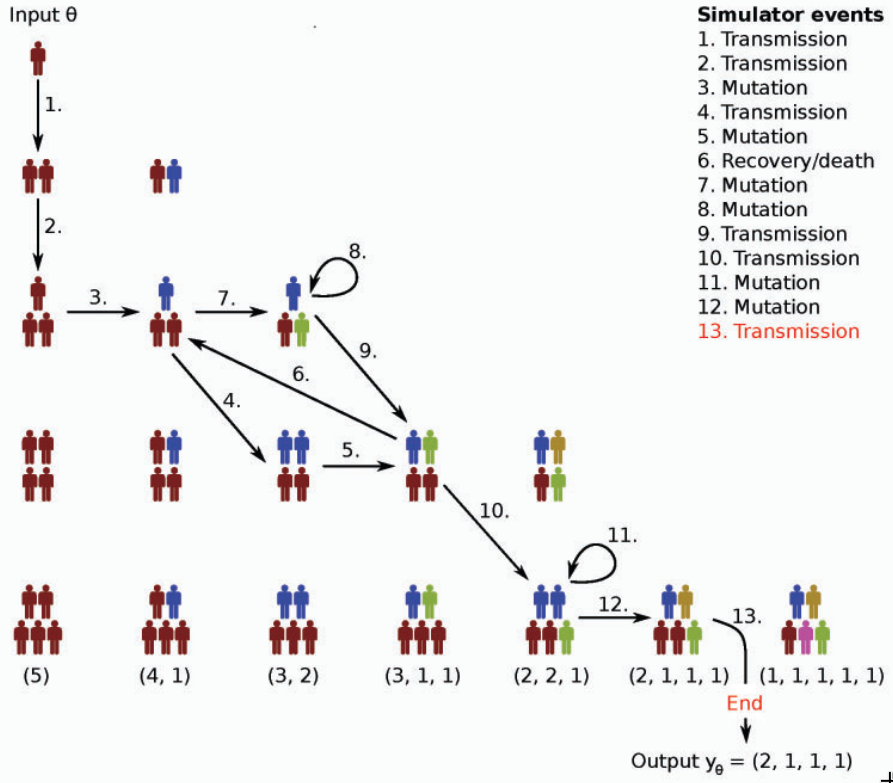
\includegraphics[width=0.75\textwidth]{./Thesis/images/chapter1/tuber_model_1.png}
    \end{center}
    \caption{Depiction of a random example from the tuberculosis
      spreading process. The image has been taken from
      \autocite{Lintusaari2017}.}
    \label{fig:tuberculosis_model}
\end{figure}

\subsubsection*{\textit{Goal of Simulation-Based Models}}

As in most Machine Learning (ML) concepts, the fundamental goal is the
derivation of one(many) parameter configuration(s) $\thetab^*$ that
\textit{describe} well the data i.e.\ generate samples
$M_r(\thetab^*)$ that are as close as possible to the observed data
$\data$. In our case, following the approach of Bayesian Machine
Learning, we treat the parameters of interest $\thetab$ as random
variables and we try to \textit{infer} a posterior distribution
$p(\thetab|\data)$ on them. 

\subsubsection*{\textit{Robust Optimisation Monte Carlo (ROMC) method}}

The ROMC method~\autocite{Ikonomov2019} is very a recent
likelihood-free approach; its fundamental idea is the transformation
of the stochastic data generation process $M_r(\thetab)$ to a
deterministic mapping $g_i(\thetab)$, by sampling the variables that
produce the randomness $\vb_i \sim p(\V)$. Formally, in every
stochastic process the randomness is influenced by a vector of random
variables $\V$, whose state is unknown before the execution of the
simulation; sampling the state makes the procedure deterministic,
namely $g_i(\thetab) = M_d(\thetab, \V=\vb_i)$. This approach
initially introduced at \autocite{Meeds2015} with the title
\textit{Optimisation Monte Carlo (OMC)}. The ROMC extended this
approach by resolving a fundamental failure-mode of OMC\@. The ROMC
describes a methodology for approximating the posterior through a
series of steps, without explicitly enforcing which algorithms must be
utilised for each step\footnote{The implementation chooses a specific
  algorithm for each task, but this choice has just a demonstrative
  value; any appropriate algorithm can be used instead.}; in this
sense, it can be thought as a meta-algorithm.

\subsubsection*{\textit{Implementation}}

The most important contribution of this work is the implementation of
the ROMC method in the Python package Engine for Likelihood-Free
Inference (ELFI) \autocite{1708.00707}. Since the method has been
published quite recently, it has not been implemented by now in any ML
software. This work attempts to provide the research community with a
robust and extensible implementation for further experimentation.
